% $Author: skashani $
% $Date: 2017/02/18 17:58:10 $
% $Revision: 1.0 $
%
%=============================================================================
\documentclass[lab]{course}

\usepackage{caption}
\usepackage{dirtree}
\usepackage[binary-units=true]{siunitx}
\usepackage{subcaption}
\usepackage{tikz}
%=============================================================================
\begin{document}

% Listing customizations =====================================================
\lstset{language=VHDL}
\lstset{showstringspaces=false}
\lstset{captionpos=b}
\lstset{moredelim=**[is][{\btHL[fill=red!15]}]{@}{@}}

% Overlay highlighting of modified listings code =============================
\makeatletter
\newenvironment{btHighlight}[1][]
{\begingroup\tikzset{bt@Highlight@par/.style={#1}}\begin{lrbox}{\@tempboxa}}
{\end{lrbox}\bt@HL@box[bt@Highlight@par]{\@tempboxa}\endgroup}

\newcommand\btHL[1][]{%
  \begin{btHighlight}[#1]\bgroup\aftergroup\bt@HL@endenv%
}
\def\bt@HL@endenv{%
  \end{btHighlight}%
  \egroup
}
\newcommand{\bt@HL@box}[2][]{%
  \tikz[#1]{%
    \pgfpathrectangle{\pgfpoint{1pt}{0pt}}{\pgfpoint{\wd #2}{\ht #2}}%
    \pgfusepath{use as bounding box}%
    \node[anchor=base west, fill=orange!30,outer sep=0pt,inner xsep=1pt, inner ysep=0pt, rounded corners=3pt, minimum height=\ht\strutbox+1pt,#1]{\raisebox{1pt}{\strut}\strut\usebox{#2}};
  }%
}
\makeatother

% ============================================================================
\setlength\parindent{0pt}

\rcsInfo $Id: vhdl_testbench_tutorial.tex,v 1.0 2017/02/18 17:58:10 skashani Exp $

\title{%
  VHDL Testbench Tutorial}
\subtitle{%
  }
\learninggoal{% compulsory
  Learning how to write a testbench in VHDL.}
\requirements{% optional
  ModelSim.}
\createdby{% optional
  Sahand Kashani-Akhavan.}
% \modifiedby{% optional
%   An Other.}
\maketitle

%=============================================================================
\sloppy % bad practice but handy...

%=============================================================================

\begin{section}{Introduction}
    An engineer's job does not stop after having created a ``solution'' to a specific problem, but he/she must also be able to demonstrate, to various degrees of certitude, that the solution is \emph{correct}. This statement is equally valid in both software \& hardware engineering, but it is especially important in the hardware domain, as errors can generally not be fixed once a product has been shipped to customers! \\

    When describing digital circuits in VHDL, one generally tests the correctness of their implementation with a VHDL \emph{testbench}. A testbench is an \emph{non-synthesizable} VHDL file which iteratively applies a sequence of controlled inputs to a circuit and compares its concrete output against the expected output. If a mismatch is detected, an error is displayed in the VHDL simulator's log which can then be consulted to help direct a designer search for the problem in the circuit's RTL description. \\

    This tutorial introduces readers to the craft of writing simple VHDL testbenches. We start with an empty VHDL testbench file and iteratively explain our thought process and how it affects the way we construct the testbench. We start with a simple testbench for a combinatorial circuit, then move on towards a more complicated testbench for a sequential circuit. \\

    For simplicity, we will introduce \emph{black box} testing. This method tests a circuit by considering it is concealed in a black box, with only its interface visible to the person testing the system. It allows one to abstract away the implementation details of the circuit and only test its behaviour at its interface. By recursively performing black box testing on all subcircuits used in larger designs, we can, with high confidence, compose systems which are correct by construction. \\

    Note that we will not be performing \emph{exhaustive} testing, which means we will not test our circuits against all possible input combinations, but rather against a carefully-chosen set of \emph{test vectors}. The number of input combinations grows exponentially with the size of a circuit's inputs, so it quickly becomes infeasible to try all combinations (unless you are willing to wait several hours for the result of a simulation).
\end{section}

\clearpage

\begin{section}{Victims / test subjects}
    We will be testing two RTL designs of a generic N-bit adder:

    \begin{enumerate}
        \item Combinatorial ripple-carry adder (Figure~\ref{fig:adder_combinatorial_interface}.)
        \item Sequential adder (Figure~\ref{fig:adder_sequential_interface}.)
    \end{enumerate}

    Each design is based upon the implementation of a 1-bit combinatorial full-adder. We assume the 1-bit full-adder is correct, so we will not be explicitly testing it. \\

    \begin{figure*}[!h]
        \centering
        \begin{subfigure}[t]{0.3\textwidth}
            \centering
            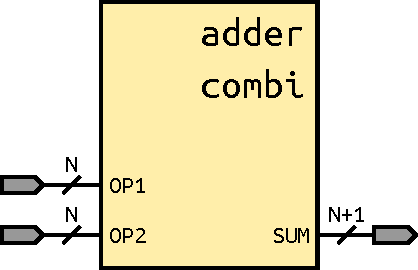
\includegraphics[width=1.0\textwidth]{figs/adder_combinatorial_interface.pdf}
            \caption{Combinatorial adder}
            \label{fig:adder_combinatorial_interface}
        \end{subfigure}
        \hspace{1em}
        \begin{subfigure}[t]{0.3\textwidth}
            \centering
            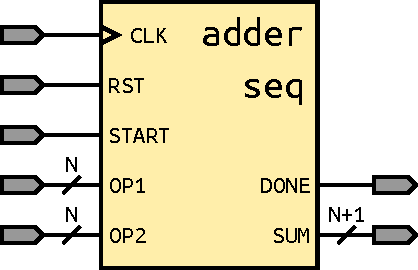
\includegraphics[width=1.0\textwidth]{figs/adder_sequential_interface.pdf}
            \caption{Sequential adder}
            \label{fig:adder_sequential_interface}
        \end{subfigure}
        \caption{Adders}
    \end{figure*}

    Note that the component being tested is often called the \emph{Design Under Test (DUT)}.

\end{section}

\begin{section}{Setup}
    \begin{subsection}{Project structure}
        Download the provided template and extract it somewhere where the directory path does \emph{not contain any spaces}. You should obtain the directory tree shown below: \\

        \dirtree{%
            .1 vhdl\_testbench\_tutorial/.
            .2     modelsim/.
            .2     testbench/.
            .3         tb\_adder\_combinatorial.vhd.
            .3         tb\_adder\_sequential.vhd.
            .2     vhdl/.
            .3         adder\_combinatorial.vhd.
            .3         adder\_sequential.vhd.
            .3         full\_adder.vhd.
        }

        \begin{enumerate}
            \item The \textbf{modelsim} folder will be used by ModelSim for its working directory.
            \item The \textbf{testbench} folder contains 100\% empty files in which we will write our testbenches for the combinatorial and sequential adders.
            \item The \textbf{vhdl} folder contains the RTL designs of our 2 adders and of the 1-bit full-adder on which they are based.
        \end{enumerate}
    \end{subsection}

    \begin{subsection}{ModelSim setup}
        \begin{enumerate}
            \item Launch ModelSim and create a new project with \verb+File > New > Project...+

            \item Name the project \verb+vhdl_testbench_tutorial+ and choose the \textbf{modelsim} folder from the extracted archive for the \verb+Project Location+ (Figure~\ref{fig:create_project})

            \item Click on the \verb+Add Existing File+ button and add all files in the \textbf{vhdl} and \textbf{testbench} directories to the project (Figure~\ref{fig:add_files_to_project}).

                \begin{figure*}[!h]
                    \centering
                    \begin{subfigure}[t]{0.45\textwidth}
                        \centering
                        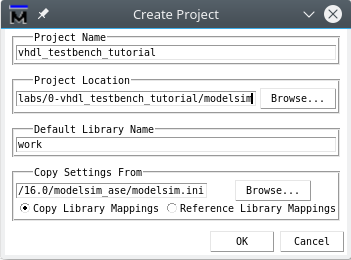
\includegraphics[width=0.9\textwidth]{figs/create_project.png}
                        \caption{Create project}
                        \label{fig:create_project}
                    \end{subfigure}
                    \hspace{1em}
                    \begin{subfigure}[t]{0.40\textwidth}
                        \centering
                        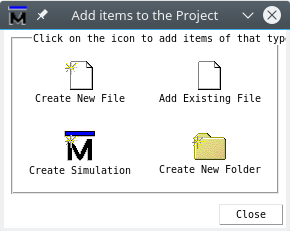
\includegraphics[width=0.9\textwidth]{figs/add_files_to_project.png}
                        \caption{Add items files to the project}
                        \label{fig:add_files_to_project}
                    \end{subfigure}
                    \begin{subfigure}[t]{1.0\textwidth}
                        \centering
                        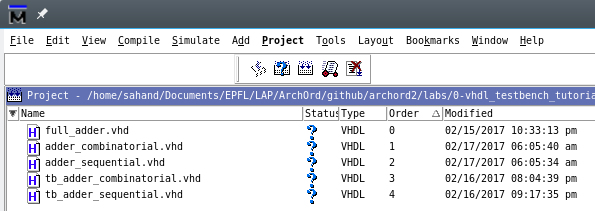
\includegraphics[width=0.825\textwidth]{figs/files_added_to_project.png}
                        \caption{Files added to project}
                        \label{fig:files_added_to_project}
                    \end{subfigure}
                    \caption{ModelSim project creation}
                \end{figure*}

            \item Click on the 
\includegraphics[height=11pt]{figs/compile_all_icon.png} icon to compile all sources. The RTL files will compile successfully, but the testbenches will fail to compile (Figure~\ref{fig:compiling_with_empty_testbenches}). This is normal as the testbench files are empty, so ModelSim does not detect any entity to compile.

                \begin{figure}[!h]
                    \begin{centering}
                        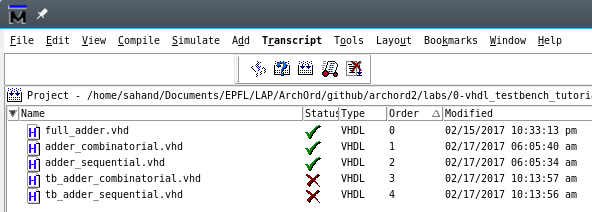
\includegraphics[width=0.825\textwidth]{figs/compiling_with_empty_testbenches.png}
                        \caption{Compiling all files (empty testbenches)}
                        \label{fig:compiling_with_empty_testbenches}
                    \end{centering}
                \end{figure}

                The ModelSim project is now set up, so we can get to writing the testbenches.
        \end{enumerate}
    \end{subsection}
\end{section}

\clearpage

\begin{section}{Testing the combinatorial adder}
    We will now write, from scratch, the testbench for the combinatorial adder. All code presented in this section is to be written in \verb+testbench/tb_adder_combinatorial.vhd+.

    \begin{subsection}{Minimum testbench}
        ModelSim complains about the fact the testbench is empty, so let's begin by filling it up with the minimum code needed to compile. \\

        All VHDL files must have an \emph{entity}, so we must write one for this testbench. An entity represents the input and output ports of a component. This makes sense if the VHDL file is describing some RTL design, but it doesn't make much sense in the case of a testbench. Indeed, a testbench is not a ``component'' which will be used in a design, but merely a simple VHDL file which is used to provide inputs to, and monitor the outputs from the DUT (the combinatorial adder in this case). So the testbench essentially has an \emph{empty} entity.

        \begin{lstlisting}[caption={Minimum testbench (only empty entity)}, label={lst:combinatorial_minimum_testbench}]
entity tb_adder_combinatorial is
end tb_adder_combinatorial;
        \end{lstlisting}
    \end{subsection}

    ModelSim should now successfully compile this testbench. \\

    We would like to actually do something useful with the testbench, so we need to add an \emph{architecture}, as well as include the libraries containing various data types we are interested in manipulating (\verb+std_logic+, \verb+std_logic_vector+, \verb+integer+, \ldots).

    \begin{lstlisting}[caption={Add libraries \& empty architecture}, label={lst:combinatorial_add_libraries_and_empty_architecture}]
@library ieee;@
@use ieee.std_logic_1164.all;@
@use ieee.numeric_std.all;@

entity tb_adder_combinatorial is
end tb_adder_combinatorial;

@architecture test of tb_adder_combinatorial is@
@begin@
@end architecture test;@
    \end{lstlisting}

    \clearpage

    \begin{subsection}{Instantiating the DUT}
        \label{sec:combinatorial_instantiating_dut}
        In order to test a component, we must have access to it. So the next step is to take the DUT, instantiate it, and wire it into the testbench. After this step, we would be able to interact with the DUT as if it were a component in the ``design'' (although we are not designing anything here, just testing). \\

        Wiring the DUT into the testbench requires information about its entity. The combinatorial adder's entity is presented in Listing~\ref{lst:adder_combinatorial_entity}. Note that the DUT is \emph{generic}: at instantiation time, the component can be configured with a specific width depending on the value provided in its \verb+N_BITS+ parameter.

        \begin{lstlisting}[caption={\texttt{adder\_combinatorial} entity}, label={lst:adder_combinatorial_entity}]
entity adder_combinatorial is
    generic(
        N_BITS : positive range 2 to positive'right  -- Operand size in bits
    );
    port(
        OP1 : in  std_logic_vector(N_BITS - 1 downto 0);  -- N-bit input.
        OP2 : in  std_logic_vector(N_BITS - 1 downto 0);  -- N-bit input.
        SUM : out std_logic_vector(N_BITS downto 0)  -- (N+1)-bit output.
    );
end entity adder_combinatorial;
        \end{lstlisting}

        We extract the relevant information from the DUT's entity and update the testbench \emph{architecture} as follows:

        \begin{enumerate}
            \item Create a \emph{constant} for every \emph{generic} parameter in the DUT's entity. You must also assign a value to the constant, as it will be used to instantiate the DUT with the configuration we want to test. We chose to implement a 4-bit adder.
            \item Create a \emph{signal} for every \emph{port} in the DUT's entity.
        \end{enumerate}

        Finally, we instantiate the DUT and wire it into the testbench with the signals created above.

        \begin{lstlisting}[caption={Instantiate DUT}, label={lst:combinatorial_instantiate_dut}]
library ieee;
use ieee.std_logic_1164.all;
use ieee.numeric_std.all;

entity tb_adder_combinatorial is
end tb_adder_combinatorial;

architecture test of tb_adder_combinatorial is

    -- adder_combinatorial GENERICS
    @constant N_BITS : positive range 2 to positive'right := 4;@

    -- adder_combinatorial PORTS
    @signal OP1 : std_logic_vector(N_BITS - 1 downto 0);@
    @signal OP2 : std_logic_vector(N_BITS - 1 downto 0);@
    @signal SUM : std_logic_vector(N_BITS downto 0);@

begin

    -- Instantiate DUT
    @dut : entity work.adder_combinatorial@
    @generic map(N_BITS => N_BITS)@
    @port map(OP1 => OP1,@
             @OP2 => OP2,@
             @SUM => SUM);@

end architecture test;
        \end{lstlisting}
    \end{subsection}

    \clearpage

    \begin{subsection}{Feeding inputs to the DUT}
        Now that the DUT is instantiated and wired into the testbench, we can start feeding it inputs to make the circuit actually do something.

        \begin{subsubsection}{Basic input feeding}
            \label{sec:combinatorial_basic_input_feeding}
            Let's go over what we are trying to achieve to see how to write the part of the testbench responsible for feeding data to the DUT. We would like to feed test vectors in \emph{sequence} to the unit, something like the execution below:

            \begin{enumerate}
                \item Supply inputs \verb+OP1+ and \verb+OP2+ from vector 1.
                \item Check output \verb+SUM+ from vector 1.
                \item Supply inputs \verb+OP1+ and \verb+OP2+ from vector 2.
                \item Check output \verb+SUM+ from vector 2.
                \item \ldots
            \end{enumerate}

            In VHDL, recall that processes execute in \emph{parallel} among each other, but the statements within each process execute in \emph{sequence}. This observation is key to writing the input-feeding part of the testbench: we can provide all inputs in a single process, separated by time intervals, and each vector will be executed one after the other until there no longer are any statements left in the process. It may be complicated to see why this works in words, so let's look at a concrete example to see how this all works.

            \begin{lstlisting}[caption={Simulation process (basic)}, label={lst:combinatorial_simulation_process_1_test_vector}]
library ieee;
use ieee.std_logic_1164.all;
use ieee.numeric_std.all;

entity tb_adder_combinatorial is
end tb_adder_combinatorial;

architecture test of tb_adder_combinatorial is

    -- "Time" that will elapse between test vectors we submit to the component.
    @constant TIME_DELTA : time := 100 ns;@

    -- adder_combinatorial GENERICS
    constant N_BITS : positive range 2 to positive'right := 4;

    -- adder_combinatorial PORTS
    signal OP1 : std_logic_vector(N_BITS - 1 downto 0);
    signal OP2 : std_logic_vector(N_BITS - 1 downto 0);
    signal SUM : std_logic_vector(N_BITS downto 0);

begin

    -- Instantiate DUT
    dut : entity work.adder_combinatorial
    generic map(N_BITS => N_BITS)
    port map(OP1 => OP1,
             OP2 => OP2,
             SUM => SUM);

    -- Test adder_combinatorial
    @simulation : process@
    @begin@
        -- Assign values to circuit inputs.
        @OP1 <= "0001";@ -- 1
        @OP2 <= "0101";@ -- 5

        -- OP1 and OP2 are NOT yet assigned. We have to wait for some time
        -- for the simulator to "propagate" their values. Any infinitesimal
        -- period would work here since we are testing a combinatorial
        -- circuit.
        @wait for TIME_DELTA;@

        -- Assign values to circuit inputs.
        @OP1 <= "0011";@ -- 3
        @OP2 <= "0010";@ -- 2

        -- OP1 and OP2 are NOT yet assigned. We have to wait for some time
        -- for the simulator to "propagate" their values. Any infinitesimal
        -- period would work here since we are testing a combinatorial
        -- circuit.
        @wait for TIME_DELTA;@
    @end process simulation;@

end architecture test;
            \end{lstlisting}
        \end{subsubsection}

        Notice that the process does \emph{not} have a sensitivity list. In VHDL, a process must either have a sensitivity list, or a \verb+wait+ statement. A testbench is not an RTL design, so it is not ``sensitive'' to any input signals. A testbench instead ``controls'' time to supply inputs at appropriate points, so the process contains 2 \verb+wait+ statements to propagate the 2 input vectors instead of a sensitivity list. \\

        Let's simulate our current testbench and see what we get.

        \begin{enumerate}
            \item Click on the 
\includegraphics[height=11pt]{figs/compile_all_icon.png} icon to compile all sources. You should get something similar to Figure~\ref{fig:compiling_with_combinatorial_testbench}. Recall that the testbench for the sequential adder is not written yet, so it is normal it fails to compile.

            \begin{figure}[!h]
                \begin{centering}
                    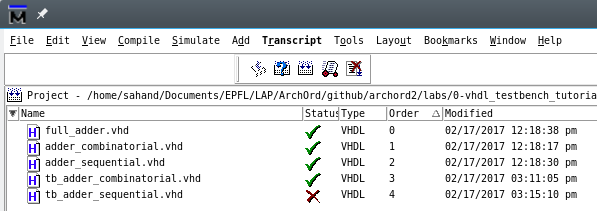
\includegraphics[width=0.85\textwidth]{figs/compiling_with_combinatorial_testbench.png}
                    \caption{Compiling all testbenches}
                    \label{fig:compiling_with_combinatorial_testbench}
                \end{centering}
            \end{figure}

            \item Go to \verb+Simulate > Start Simulation...+

            \item Select \verb+work > tb_adder_combinatorial+, then press \verb+OK+ (Figure~\ref{fig:start_tb_adder_combinatorial_simulation}).

            \begin{figure}[!h]
                \begin{centering}
                    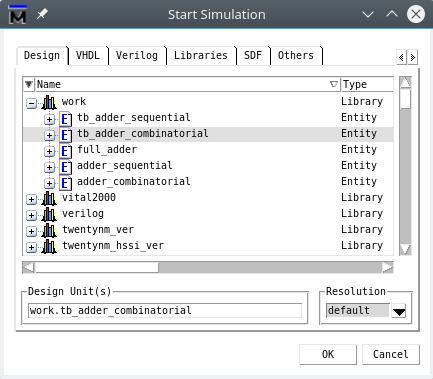
\includegraphics[width=0.50\textwidth]{figs/start_tb_adder_combinatorial_simulation.png}
                    \caption{Start simulation}
                    \label{fig:start_tb_adder_combinatorial_simulation}
                \end{centering}
            \end{figure}

            \item In the \verb+sim+ tab, click on \verb+tb_adder_combinatorial+ (Figure~\ref{fig:sim_tab_tb_adder_combinatorial_simulation}).

            \begin{figure}[!h]
                \begin{centering}
                    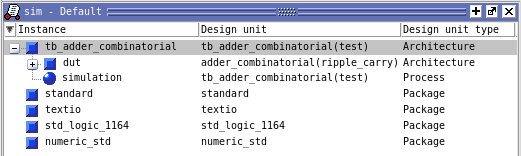
\includegraphics[width=0.75\textwidth]{figs/sim_tab_tb_adder_combinatorial_simulation.png}
                    \caption{Simulation tab}
                    \label{fig:sim_tab_tb_adder_combinatorial_simulation}
                \end{centering}
            \end{figure}

            \item Go to \verb+Add > To Wave > All items in region+.

            \item Finally, in the simulation transcript, type \verb+restart -f; run 600 ns;+ (Figure~\ref{fig:waveform_combinatorial_transcript_basic_version}). A waveform window should appear with the result of the simulation (Figure~\ref{fig:waveform_combinatorial_process_reexecutes}).

            \begin{figure}[!h]
                \begin{centering}
                    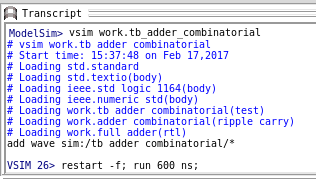
\includegraphics[width=0.5\textwidth]{figs/waveform_combinatorial_transcript_basic_version.png}
                    \caption{Transcript}
                    \label{fig:waveform_combinatorial_transcript_basic_version}
                \end{centering}
            \end{figure}

            \begin{figure}[!h]
                \begin{centering}
                    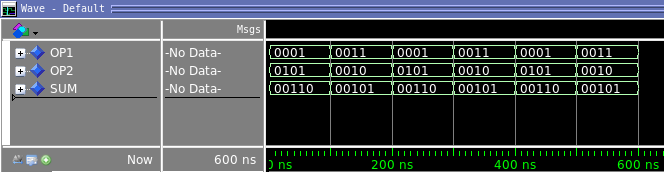
\includegraphics[width=0.85\textwidth]{figs/waveform_combinatorial_process_reexecutes.png}
                    \caption{Waveform (repetitive input feeding)}
                    \label{fig:waveform_combinatorial_process_reexecutes}
                \end{centering}
            \end{figure}

            The results look correct, i.e. $1 + 5 = 6$ and $3 + 2 = 5$, so at least the circuit is behaving correctly with these 2 input vectors. However, notice that the simulation is ``looping'' and is applying the two input vectors 3 times. Recall how processes work in VHDL. A process executes all its statements sequentially, then restarts. In the testbench, the simulation process uses 2 \verb+wait+ statements for a total of \SI{200}{\nano\second} of simulation time. Since we asked for a \SI{600}{\nano\second} simulation, the process had enough time to restart 3 times.
        \end{enumerate}

        \clearpage

        \begin{subsubsection}{Automatic simulation termination}
            In Figure~\ref{fig:waveform_combinatorial_transcript_basic_version}, we saw that we had to manually provide the simulation interval, \SI{600}{\nano\second}, to ModelSim. Manually selecting the time interval is error-prone, as one may accidentally supply an interval too short for all test vectors to pass through the DUT, or too long and unnecessarily re-executing test vectors which have already passed through the DUT. \\

            It would be nice if the simulator could let the simulation run for as long as needed, i.e. until all test vectors have passed through the DUT, then automatically halt the simulation. ModelSim has a command specifically for this purpose: \verb+run -all+. Instead of specifying a time interval, the \verb+-all+ flag instructs ModelSim to continue simulating as long as events are scheduled for simulation. Therefore, one way to halt the simulation is to cause processes \emph{not} to restart once they have finished all their statements. This can be achieved by placing an \emph{indefinite} \verb+wait+ statement at the end of the simulation process, after all the test vectors have passed through the DUT.

            \begin{lstlisting}[caption={Indefinite \texttt{wait} statement added to simulation process}, label={lst:combinatorial_indefinite_wait_statement_added_to_simulation_process}]
library ieee;
use ieee.std_logic_1164.all;
use ieee.numeric_std.all;

entity tb_adder_combinatorial is
end tb_adder_combinatorial;

architecture test of tb_adder_combinatorial is

    -- "Time" that will elapse between test vectors we submit to the component.
    constant TIME_DELTA : time := 100 ns;

    -- adder_combinatorial GENERICS
    constant N_BITS : positive range 2 to positive'right := 4;

    -- adder_combinatorial PORTS
    signal OP1 : std_logic_vector(N_BITS - 1 downto 0);
    signal OP2 : std_logic_vector(N_BITS - 1 downto 0);
    signal SUM : std_logic_vector(N_BITS downto 0);

begin

    -- Instantiate DUT
    dut : entity work.adder_combinatorial
    generic map(N_BITS => N_BITS)
    port map(OP1 => OP1,
             OP2 => OP2,
             SUM => SUM);

    -- Test adder_combinatorial
    simulation : process
    begin
        -- Assign values to circuit inputs.
        OP1 <= "0001"; -- 1
        OP2 <= "0101"; -- 5

        -- OP1 and OP2 are NOT yet assigned. We have to wait for some time
        -- for the simulator to "propagate" their values. Any infinitesimal
        -- period would work here since we are testing a combinatorial
        -- circuit.
        wait for TIME_DELTA;

        -- Assign values to circuit inputs.
        OP1 <= "0011"; -- 3
        OP2 <= "0010"; -- 2

        -- OP1 and OP2 are NOT yet assigned. We have to wait for some time
        -- for the simulator to "propagate" their values. Any infinitesimal
        -- period would work here since we are testing a combinatorial
        -- circuit.
        wait for TIME_DELTA;

        -- Make this process wait indefinitely (it will never re-execute from
        -- its beginning again).
        @wait;@
    end process simulation;

end architecture test;
            \end{lstlisting}

            If we now recompile and relaunch the simulation, we should obtain the output shown in Figure~\ref{fig:waveform_combinatorial_process_automatically_terminates}.

            \begin{figure*}[!h]
                \centering
                \begin{subfigure}[t]{0.4\textwidth}
                    \centering
                    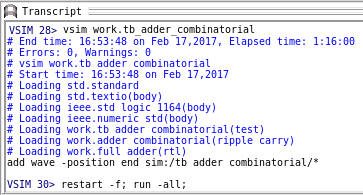
\includegraphics[width=1.0\textwidth]{figs/waveform_combinatorial_transcript_automatic_termination.png}
                    \caption{Transcript}
                    \label{fig:waveform_combinatorial_transcript_automatically_terminates}
                \end{subfigure}
                \hspace{1em}
                \begin{subfigure}[t]{0.55\textwidth}
                    \centering
                    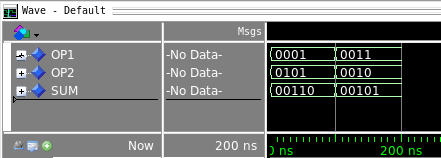
\includegraphics[width=1.0\textwidth]{figs/waveform_combinatorial_process_automatic_termination.png}
                    \caption{Waveform}
                    \label{fig:waveform_combinatorial_process_automatically_terminates}
                \end{subfigure}
                \caption{Automatic simulation termination}
            \end{figure*}
        \end{subsubsection}

        \clearpage

        \begin{subsubsection}{Avoiding code duplication}
            Listing~\ref{lst:combinatorial_indefinite_wait_statement_added_to_simulation_process} is quite simple, but we can already see that there is a fair amount of code duplication going on. Every additional test vector requires copy-pasting the code responsible for the operand assignments and the \verb+wait+ statement. Although not exhaustive, we want to test the DUT with a potentially large number of test vectors to have more confidence in its correctness. However, a large number of test vectors would cause a huge increase in the simulation process' code size, therefore making it hard to read. \\

            We handle this issue by refactoring the code used to feed a test vector into a \emph{procedure} called \verb+check_add+. Notice the type of the input arguments provided to the \verb+check_add+ procedure. We provide the operands in \verb+natural+ format instead of in \verb+std_logic_vector+. This makes it easy to create \& add test vectors, and also makes the code more readable. \\

            As a side-effect, we increased the count of test vectors from 2 to 10 for illustration purposes.

            \begin{lstlisting}[caption={Refactored test vector feeding code into a \emph{procedure} called \texttt{check\_add}}, label={lst:combinatorial_refactored_test_vector_feeding_code}]
library ieee;
use ieee.std_logic_1164.all;
use ieee.numeric_std.all;

entity tb_adder_combinatorial is
end tb_adder_combinatorial;

architecture test of tb_adder_combinatorial is

    -- "Time" that will elapse between test vectors we submit to the component.
    constant TIME_DELTA : time := 100 ns;

    -- adder_combinatorial GENERICS
    constant N_BITS : positive range 2 to positive'right := 4;

    -- adder_combinatorial PORTS
    signal OP1 : std_logic_vector(N_BITS - 1 downto 0);
    signal OP2 : std_logic_vector(N_BITS - 1 downto 0);
    signal SUM : std_logic_vector(N_BITS downto 0);

begin

    -- Instantiate DUT
    dut : entity work.adder_combinatorial
    generic map(N_BITS => N_BITS)
    port map(OP1 => OP1,
             OP2 => OP2,
             SUM => SUM);

    -- Test adder_combinatorial
    simulation : process

        @procedure check_add(constant in1 : in natural;@
                            @constant in2 : in natural) is@
        @begin@
            -- Assign values to circuit inputs.
            @OP1 <= std_logic_vector(to_unsigned(in1, OP1'length));@
            @OP2 <= std_logic_vector(to_unsigned(in2, OP2'length));@

            -- OP1 and OP2 are NOT yet assigned. We have to wait for some time
            -- for the simulator to "propagate" their values. Any infinitesimal
            -- period would work here since we are testing a combinatorial
            -- circuit.
            @wait for TIME_DELTA;@
        @end procedure check_add;@

    begin

        -- Check test vectors
        @check_add(12, 8);@
        @check_add(10, 6);@
        @check_add(4, 1);@
        @check_add(11, 7);@
        @check_add(10, 13);@
        @check_add(8, 7);@
        @check_add(1, 9);@
        @check_add(7, 3);@
        @check_add(1, 4);@
        @check_add(8, 0);@

        -- Make this process wait indefinitely (it will never re-execute from
        -- its beginning again).
        wait;
    end process simulation;

end architecture test;
            \end{lstlisting}

            Recompiling and relaunching the simulation (\verb+restart -f; run -all;+) results in a waveform with many more test vectors being shown (Figure~\ref{fig:waveform_combinatorial_process_avoid_code_duplication}).

            \begin{figure}[!h]
                \begin{centering}
                    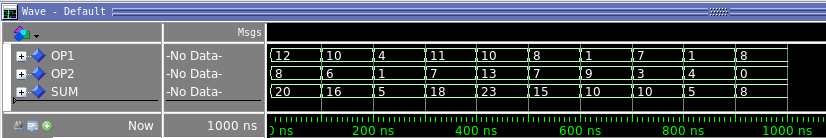
\includegraphics[width=1.0\textwidth]{figs/waveform_combinatorial_process_avoid_code_duplication.png}
                    \caption{Waveform (many test vectors). Note that, by default, ModelSim displays signals in binary on a waveform. You can modify the display radix of various signals by selecting the signals and going to \texttt{Wave > Format > Radix}. The \texttt{Unsigned} radix is used in this waveform.}
                    \label{fig:waveform_combinatorial_process_avoid_code_duplication}
                \end{centering}
            \end{figure}
        \end{subsubsection}

        \clearpage

        \begin{subsubsection}{Self-checking testbench}
            Listing~\ref{lst:combinatorial_refactored_test_vector_feeding_code} is easy to read and to modify, but there is one last thing which is quite cumbersome: verifying the DUT's outputs. With the current system, a human must visually check the DUT's outputs for correctness on the simulation waveform. Although not a difficult task, it is quite annoying and error-prone to have someone manually verify a waveform containing hundreds, perhaps thousands, of test vectors. \\

            It would be great if the user could modify the definition of a test vector to not only include DUT inputs, but also its \emph{expected} output. We could then modify the testbench such that it automatically compares the output of the DUT with the expected output provided in the test vector. Nobody would then have to manually check the results for correctness. This type of testbench is commonly called a \emph{self-checking} testbench. We apply the idea in Listing~\ref{lst:combinatorial_self_checking_testbench}. \\

            Notice how we use an assertion to compare the DUT output with the expected output provided in the test vector. The VHDL \verb+assert+ statement is followed by:

            \begin{enumerate}
                \item A \verb+report+ statement and a string describing the error.
                \item A \verb+severity+ statement and a severity level. VHDL supports 4 severity levels (\verb+note+, \verb+warning+, \verb+error+, \verb+failure+) and simulators can be configured to react to each severity level in different ways. We do not use this feature, but it is good to be aware of.
            \end{enumerate}

            \begin{lstlisting}[caption={Self-checking testbench: updated \texttt{check\_add} procedure to automatically compare DUT output against expected output provided in test vector}, label={lst:combinatorial_self_checking_testbench}]
library ieee;
use ieee.std_logic_1164.all;
use ieee.numeric_std.all;

entity tb_adder_combinatorial is
end tb_adder_combinatorial;

architecture test of tb_adder_combinatorial is

    -- "Time" that will elapse between test vectors we submit to the component.
    constant TIME_DELTA : time := 100 ns;

    -- adder_combinatorial GENERICS
    constant N_BITS : positive range 2 to positive'right := 4;

    -- adder_combinatorial PORTS
    signal OP1 : std_logic_vector(N_BITS - 1 downto 0);
    signal OP2 : std_logic_vector(N_BITS - 1 downto 0);
    signal SUM : std_logic_vector(N_BITS downto 0);

begin
    -- Instantiate DUT
    dut : entity work.adder_combinatorial
    generic map(N_BITS => N_BITS)
    port map(OP1 => OP1,
             OP2 => OP2,
             SUM => SUM);

    -- Test adder_combinatorial
    simulation : process

        procedure check_add(constant in1          : in natural;
                            constant in2          : in natural;
                            constant res_expected : in natural) is
            variable res : natural;
        begin
            -- Assign values to circuit inputs.
            OP1 <= std_logic_vector(to_unsigned(in1, OP1'length));
            OP2 <= std_logic_vector(to_unsigned(in2, OP2'length));

            -- OP1 and OP2 are NOT yet assigned. We have to wait for some time
            -- for the simulator to "propagate" their values. Any infinitesimal
            -- period would work here since we are testing a combinatorial
            -- circuit.
            wait for TIME_DELTA;

            -- Check output against expected result.
            @res := to_integer(unsigned(SUM));@
            @assert res = res_expected@
            @report "Unexpected result: " &@
                   @"OP1 = " & integer'image(in1) & "; " &@
                   @"OP2 = " & integer'image(in2) & "; " &@
                   @"SUM = " & integer'image(res) & "; " &@
                   @"SUM_expected = " & integer'image(res_expected)@
            @severity error;@
        end procedure check_add;

    begin

        -- Check test vectors against expected outputs
        check_add(12, 8, 20);
        check_add(10, 6, 16);
        check_add(4, 1, 5);
        check_add(11, 7, 18);
        check_add(10, 13, 23);
        check_add(8, 7, 15);
        check_add(1, 9, 10);
        check_add(7, 3, 10);
        check_add(1, 4, 5);
        check_add(8, 0, 8);

        -- Make this process wait indefinitely (it will never re-execute from
        -- its beginning again).
        wait;
    end process simulation;

end architecture test;
            \end{lstlisting}
        \end{subsubsection}
    \end{subsection}
\end{section}

\clearpage

\begin{section}{Testing the sequential adder}
    We will now write, from scratch, the testbench for the sequential adder. All code presented in this section is to be written in \verb+testbench/tb_adder_sequential.vhd+.

    \begin{subsection}{Instantiating the DUT}
        Let's start by instantiating the DUT and wiring it into the testbench. We use the same algorithm described in Section~\ref{sec:combinatorial_instantiating_dut} to obtain Listing~\ref{lst:sequential_instantiate_dut}.

        \begin{lstlisting}[caption={Instantiate DUT}, label={lst:sequential_instantiate_dut}]
library ieee;
use ieee.std_logic_1164.all;
use ieee.numeric_std.all;

entity tb_adder_sequential is
end tb_adder_sequential;

architecture test of tb_adder_sequential is

    -- adder_sequential GENERICS
    constant N_BITS : positive range 2 to positive'right := 4;

    -- adder_sequential PORTS
    signal CLK   : std_logic;
    signal RST   : std_logic;
    signal START : std_logic;
    signal OP1   : std_logic_vector(N_BITS - 1 downto 0);
    signal OP2   : std_logic_vector(N_BITS - 1 downto 0);
    signal SUM   : std_logic_vector(N_BITS downto 0);
    signal DONE  : std_logic;

begin

    -- Instantiate DUT
    dut : entity work.adder_sequential
    generic map(N_BITS => N_BITS)
    port map(CLK   => CLK,
             RST   => RST,
             START => START,
             OP1   => OP1,
             OP2   => OP2,
             SUM   => SUM,
             DONE  => DONE);

end architecture test;
        \end{lstlisting}
    \end{subsection}

    \clearpage

    \begin{subsection}{Generating a clock signal}
        The sequential adder is a synchronous component as it is sensitive to a clock. We saw in Section~\ref{sec:combinatorial_basic_input_feeding} that, for simulation purposes, one can assign values to signals by using a VHDL process. We do the same in Listing~\ref{lst:sequential_process_generate_clk} specifically for generating the \verb+CLK+ input of the DUT.

        \begin{lstlisting}[caption={Add process for generating \texttt{CLK} signal}, label={lst:sequential_process_generate_clk}]
library ieee;
use ieee.std_logic_1164.all;
use ieee.numeric_std.all;

entity tb_adder_sequential is
end tb_adder_sequential;

architecture test of tb_adder_sequential is

    @constant CLK_PERIOD : time := 100 ns;@

    -- adder_sequential GENERICS
    constant N_BITS : positive range 2 to positive'right := 4;

    -- adder_sequential PORTS
    signal CLK   : std_logic;
    signal RST   : std_logic;
    signal START : std_logic;
    signal OP1   : std_logic_vector(N_BITS - 1 downto 0);
    signal OP2   : std_logic_vector(N_BITS - 1 downto 0);
    signal SUM   : std_logic_vector(N_BITS downto 0);
    signal DONE  : std_logic;

begin

    -- Instantiate DUT
    dut : entity work.adder_sequential
    generic map(N_BITS => N_BITS)
    port map(CLK   => CLK,
             RST   => RST,
             START => START,
             OP1   => OP1,
             OP2   => OP2,
             SUM   => SUM,
             DONE  => DONE);

    -- Generate CLK signal
    @clk_generation : process@
    @begin@
        @clk <= '1';@
        @wait for CLK_PERIOD / 2;@
        @clk <= '0';@
        @wait for CLK_PERIOD / 2;@
    @end process clk_generation;@

end architecture test;
        \end{lstlisting}

        Note the absence of any \emph{indefinite} \verb+wait+ statement in the \verb+clk_generation+ process. It is important that one \emph{not} use such an indefinite \verb+wait+ statement, otherwise the process would only generate a single clock pulse before halting instead of continuously generating clock pulses each time the process restarts. \\

        A consequence of this design is that one cannot use the \verb+run -all+ command in ModelSim, but must instead explicitly provide a simulation duration such as \verb+run 1000 ns+.
    \end{subsection}

    \begin{subsection}{Feeding inputs to the DUT}

        \begin{subsubsection}{Default DUT inputs}
            In Section~\ref{sec:combinatorial_basic_input_feeding}, we used a \emph{single} process for feeding inputs to the \emph{combinatorial} adder. Could we envision doing the same thing for the \emph{sequential} adder (i.e. use a \emph{single} process for generating the clock signal and the non-clock signals)? \\

            A clock signal is \emph{periodic}, whereas non-clock signals are generally \emph{non-periodic}. Recall the execution model of VHDL processes: processes execute in \emph{parallel} among each other, but the statements within each process execute in \emph{sequence}. Given this execution model, there is no way to describe the periodic behaviour of a clock parallely to the sequential behaviour of the other input signals in a \emph{single} process. \\

            However, it is possible to do so with \emph{multiple} processes. One process can periodically generate a clock signal, while another process can sequentially generate the non-clock signals which are to be fed to the DUT. The 2 processes execute in parallel, so we can correctly model the periodic and non-periodic behaviour of our 2 signal categories (clock and non-clock). \\

            Therefore, we update our testbench with a second process called \verb+simulation+ which is responsible for generating the non-clock inputs of the DUT. Our first attempt is shown in Listing~\ref{lst:sequential_process_simulation_default_values} where the testbench just assigns default values to the DUT's non-clock signals.

            \begin{lstlisting}[caption={Add \texttt{simulation} process for generating non-clock signals to the DUT. This first version only assigns default values to the non-clock signals.}, label={lst:sequential_process_simulation_default_values}]
library ieee;
use ieee.std_logic_1164.all;
use ieee.numeric_std.all;

entity tb_adder_sequential is
end tb_adder_sequential;

architecture test of tb_adder_sequential is

    constant CLK_PERIOD : time := 100 ns;

    -- adder_sequential GENERICS
    constant N_BITS : positive range 2 to positive'right := 4;

    -- adder_sequential PORTS
    signal CLK   : std_logic;
    signal RST   : std_logic;
    signal START : std_logic;
    signal OP1   : std_logic_vector(N_BITS - 1 downto 0);
    signal OP2   : std_logic_vector(N_BITS - 1 downto 0);
    signal SUM   : std_logic_vector(N_BITS downto 0);
    signal DONE  : std_logic;

begin

    -- Instantiate DUT
    dut : entity work.adder_sequential
    generic map(N_BITS => N_BITS)
    port map(CLK   => CLK,
             RST   => RST,
             START => START,
             OP1   => OP1,
             OP2   => OP2,
             SUM   => SUM,
             DONE  => DONE);

    -- Generate CLK signal
    clk_generation : process
    begin
        clk <= '1';
        wait for CLK_PERIOD / 2;
        clk <= '0';
        wait for CLK_PERIOD / 2;
    end process clk_generation;

    -- Test adder_sequential
    @simulation : process@
    @begin@

        -- Default values
        @OP1   <= (others => '0');@
        @OP2   <= (others => '0');@
        @RST   <= '0';@
        @START <= '0';@
        @wait for CLK_PERIOD;@
    @end process simulation;@

end architecture test;
            \end{lstlisting}
        \end{subsubsection}

        \begin{subsubsection}{Resetting the DUT}
            The DUT is a synchronous circuit and has an \emph{asynchronous} reset input, verb+RST+. When testing a component, it is a good practice to supply it with a reset pulse before feeding it any other inputs. This guarantees the DUT is in a valid state before we do anything. We update the \verb+simulation+ process with an \verb+async_reset+ \emph{procedure} for this.

            \begin{lstlisting}[caption={Add \emph{asynchronous} reset}, label={lst:sequential_process_simulation_async_reset}]
library ieee;
use ieee.std_logic_1164.all;
use ieee.numeric_std.all;

entity tb_adder_sequential is
end tb_adder_sequential;

architecture test of tb_adder_sequential is

    constant CLK_PERIOD : time := 100 ns;

    -- adder_sequential GENERICS
    constant N_BITS : positive range 2 to positive'right := 4;

    -- adder_sequential PORTS
    signal CLK   : std_logic;
    signal RST   : std_logic;
    signal START : std_logic;
    signal OP1   : std_logic_vector(N_BITS - 1 downto 0);
    signal OP2   : std_logic_vector(N_BITS - 1 downto 0);
    signal SUM   : std_logic_vector(N_BITS downto 0);
    signal DONE  : std_logic;

begin

    -- Instantiate DUT
    dut : entity work.adder_sequential
    generic map(N_BITS => N_BITS)
    port map(CLK   => CLK,
             RST   => RST,
             START => START,
             OP1   => OP1,
             OP2   => OP2,
             SUM   => SUM,
             DONE  => DONE);

    -- Generate CLK signal
    clk_generation : process
    begin
        clk <= '1';
        wait for CLK_PERIOD / 2;
        clk <= '0';
        wait for CLK_PERIOD / 2;
    end process clk_generation;

    -- Test adder_sequential
    simulation : process

        @procedure async_reset is@
        @begin@
            @wait until rising_edge(CLK);@
            @wait for CLK_PERIOD / 4;@
            @RST <= '1';@

            @wait for CLK_PERIOD / 2;@
            @RST <= '0';@
        @end procedure async_reset;@

    begin

        -- Default values
        OP1   <= (others => '0');
        OP2   <= (others => '0');
        RST   <= '0';
        START <= '0';
        wait for CLK_PERIOD;

        -- Reset the circuit.
        @async_reset;@
    end process simulation;

end architecture test;
            \end{lstlisting}
        \end{subsubsection}

        \begin{subsubsection}{Self-checking test vectors}

            Now that the DUT is in a valid initial state, we can start feeding it test vectors and automatically check if the output is correct. We create a \verb+check_add+ \emph{procedure} for this purpose, similarly as for the combinatorial adder.

            \begin{lstlisting}[caption={Add test vectors}, label={lst:sequential_process_simulation_test_vectors}]
library ieee;
use ieee.std_logic_1164.all;
use ieee.numeric_std.all;

entity tb_adder_sequential is
end tb_adder_sequential;

architecture test of tb_adder_sequential is

    constant CLK_PERIOD : time := 100 ns;

    -- adder_sequential GENERICS
    constant N_BITS : positive range 2 to positive'right := 4;

    -- adder_sequential PORTS
    signal CLK   : std_logic;
    signal RST   : std_logic;
    signal START : std_logic;
    signal OP1   : std_logic_vector(N_BITS - 1 downto 0);
    signal OP2   : std_logic_vector(N_BITS - 1 downto 0);
    signal SUM   : std_logic_vector(N_BITS downto 0);
    signal DONE  : std_logic;

begin

    -- Instantiate DUT
    dut : entity work.adder_sequential
    generic map(N_BITS => N_BITS)
    port map(CLK   => CLK,
             RST   => RST,
             START => START,
             OP1   => OP1,
             OP2   => OP2,
             SUM   => SUM,
             DONE  => DONE);

    -- Generate CLK signal
    clk_generation : process
    begin
        clk <= '1';
        wait for CLK_PERIOD / 2;
        clk <= '0';
        wait for CLK_PERIOD / 2;
    end process clk_generation;

    -- Test adder_sequential
    simulation : process

        procedure async_reset is
        begin
            wait until rising_edge(CLK);
            wait for CLK_PERIOD / 4;
            RST <= '1';

            wait for CLK_PERIOD / 2;
            RST <= '0';
        end procedure async_reset;

        @procedure check_add(constant in1          : in natural;@
                            @constant in2          : in natural;@
                            @constant res_expected : in natural) is@
            @variable res : natural;@
        @begin@
            -- Our circuit is sensitive to the rising edge of the CLK, so we
            -- need to be sure to assign signal values such that they are stable
            -- at the next rising edge of the CLK.
            @wait until rising_edge(CLK);@

            -- Assign values to circuit inputs.
            @OP1   <= std_logic_vector(to_unsigned(in1, OP1'length));@
            @OP2   <= std_logic_vector(to_unsigned(in2, OP2'length));@
            @START <= '1';@

            -- OP1, OP2 and START are NOT yet assigned. We have to wait for some
            -- time for the simulator to "propagate" their values. Any
            -- infinitesimal period would work for the simulator to "propagate"
            -- the values. However, our circuit is a sequential circuit
            -- sensitive to the rising edge of CLK, so we need to hold our
            -- signal assignments until the next rising edge of CLK so the
            -- circuit can see them.
            @wait until rising_edge(CLK);@

            -- Remove values from circuit inputs. The circuit works with a PULSE
            -- on its START input, which means that data on the inputs only
            -- needs to be valid when START is high.
            @OP1   <= (others => '0');@
            @OP2   <= (others => '0');@
            @START <= '0';@

            -- The circuit informs us it has finished by asserting DONE, so we
            -- can wait until we receive the signal before proceeding. DONE is
            -- asserted at the rising edge of CLK, so we (the test system) can
            -- sample the data and check its correctness.
            @wait until DONE = '1';@

            -- Check output against expected result.
            @res := to_integer(unsigned(SUM));@
            @assert res = res_expected@
            @report "Unexpected result: " &@
                   @"OP1 = " & integer'image(in1) & "; " &@
                   @"OP2 = " & integer'image(in2) & "; " &@
                   @"SUM = " & integer'image(res) & "; " &@
                   @"SUM_expected = " & integer'image(res_expected)@
            @severity error;@

            -- Wait for the circuit to go back into the IDLE state.
            @wait until DONE = '0';@
        @end procedure check_add;@

    begin

        -- Default values
        OP1   <= (others => '0');
        OP2   <= (others => '0');
        RST   <= '0';
        START <= '0';
        wait for CLK_PERIOD;

        -- Reset the circuit.
        async_reset;

        -- Check test vectors against expected outputs
        @check_add(12, 8, 20);@
    end process simulation;

end architecture test;
            \end{lstlisting}

            Let's simulate our current testbench and see what we get.

            \begin{enumerate}
                \item Click on the 
\includegraphics[height=11pt]{figs/compile_all_icon.png} icon to compile all sources. You should get something similar to Figure~\ref{fig:compiling_with_sequential_testbench}. All files should successfully compile as they now all contain valid VHDL.

                \begin{figure}[!h]
                    \begin{centering}
                        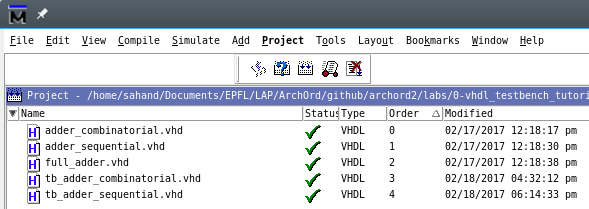
\includegraphics[width=0.85\textwidth]{figs/compiling_with_sequential_testbench.png}
                        \caption{Compiling all testbenches}
                        \label{fig:compiling_with_sequential_testbench}
                    \end{centering}
                \end{figure}

                \item Go to \verb+Simulate > Start Simulation...+

                \item Select \verb+work > tb_adder_sequential+, then press \verb+OK+ (Figure~\ref{fig:start_tb_adder_sequential_simulation}).

                \begin{figure}[!h]
                    \begin{centering}
                        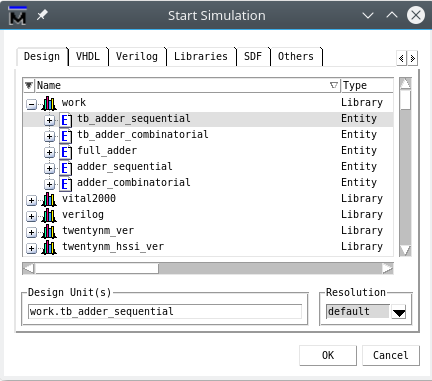
\includegraphics[width=0.50\textwidth]{figs/start_tb_adder_sequential_simulation.png}
                        \caption{Start simulation}
                        \label{fig:start_tb_adder_sequential_simulation}
                    \end{centering}
                \end{figure}

                \item In the \verb+sim+ tab, click on \verb+tb_adder_sequential+ (Figure~\ref{fig:sim_tab_tb_adder_sequential_simulation}).

                \begin{figure}[!h]
                    \begin{centering}
                        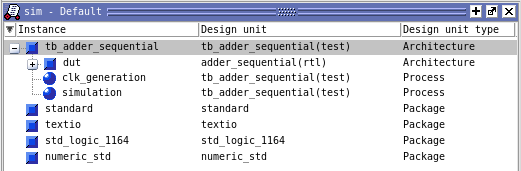
\includegraphics[width=0.75\textwidth]{figs/sim_tab_tb_adder_sequential_simulation.png}
                        \caption{Simulation tab}
                        \label{fig:sim_tab_tb_adder_sequential_simulation}
                    \end{centering}
                \end{figure}

                \item Go to \verb+Add > To Wave > All items in region+.

                \item Finally, in the simulation transcript, type \verb+restart -f; run 2000 ns;+ (Figure~\ref{fig:waveform_sequential_transcript_basic_version}). A waveform window should appear with the result of the simulation (Figure~\ref{fig:waveform_sequential_process_reexecutes}).

                \begin{figure}[!h]
                    \begin{centering}
                        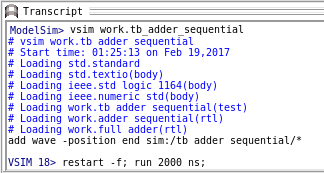
\includegraphics[width=0.5\textwidth]{figs/waveform_sequential_transcript_basic_version.png}
                        \caption{Transcript}
                        \label{fig:waveform_sequential_transcript_basic_version}
                    \end{centering}
                \end{figure}

                \begin{figure}[!h]
                    \begin{centering}
                        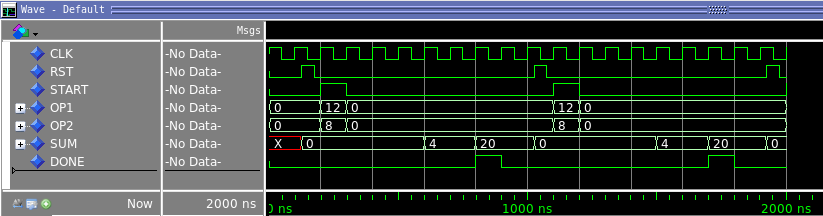
\includegraphics[width=0.85\textwidth]{figs/waveform_sequential_process_reexecutes.png}
                        \caption{Waveform (repetitive input feeding)}
                        \label{fig:waveform_sequential_process_reexecutes}
                    \end{centering}
                \end{figure}

                The results look correct:

                \begin{enumerate}
                    \item The circuit seems to be reset as the \verb+SUM+ output changes as soon as \verb+RST+ is high (recall it is an \emph{asynchronous} reset, so various registers should be reset as soon as the reset signal is high, and \emph{not} at the next rising edge of the clock signal).

                    \item The test vector $12 + 8 = 20$ is correct.
                \end{enumerate}

                However, we suffer from the ``loopy'' execution of the \verb+simulation+ process again, as was previously seen for the combinatorial adder. We will address this issue next so we can take advantage of ModelSim's practical automatic simulation termination command, \verb+run -all+.
            \end{enumerate}
        \end{subsubsection}

        \begin{subsubsection}{Automatic simulation termination}
            For the combinatorial adder, we saw how to stop a process from re-executing by means of an \emph{indefinite} \verb+wait+ statement. We would like to use the same technique to automatically halt the simulation with ModelSim's \verb+run -all+ command once all test vectors have gone through the DUT. Unfortunately, unlike for the combinatorial adder, simply adding an indefinite \verb+wait+ statement to the \verb+simulation+ process will not be sufficient for the simulation to automatically terminate. \\

            Recall the semantics of the \verb+run -all+ command: ModelSim terminates the simulation when there no longer exists any scheduled signal assignment in the testbench. If we add an indefinite \verb+wait+ statement to the \verb+simulation+ process, then this process will indeed never re-execute, causing our test vectors to only go through the DUT once (which is what we are looking for). However, the \verb+clk_generation+ process still keeps restarting, so there always will be scheduled signal assignments in the testbench. The end result is that the \verb+run -all+ command will never stop the simulation! \\

            To address this issue, we would need the \verb+clk_generation+ process to also stop scheduling any new signal assignments once all test vectors have gone through the DUT in the \verb+simulation+ process. We can achieve this by introducing a boolean \verb+sim_finished+ signal. The \verb+sim_finished+ signal is written by the \verb+simulation+ process once all test vectors have gone through the DUT, and is continuously read by the \verb+clk_generation+ process to know when to stop scheduling any new signal assignments. If the \verb+sim_finished+ signal is \verb+true+, then we can use an indefinite \verb+wait+ statement in both processes to avoid any new signal assignments from occuring, therefore allowing ModelSim to automatically terminate the simulation. \\

            Listing~\ref{lst:sequential_process_simulation_automatic_termination} shows how to use this technique.

            \begin{lstlisting}[caption={Automatic simulation termination}, label={lst:sequential_process_simulation_automatic_termination}]
library ieee;
use ieee.std_logic_1164.all;
use ieee.numeric_std.all;

entity tb_adder_sequential is
end tb_adder_sequential;

architecture test of tb_adder_sequential is

    constant CLK_PERIOD : time := 100 ns;

    -- Signal used to end simulator when we finished submitting our test cases
    @signal sim_finished : boolean := false;@

    -- adder_sequential GENERICS
    constant N_BITS : positive range 2 to positive'right := 4;

    -- adder_sequential PORTS
    signal CLK   : std_logic;
    signal RST   : std_logic;
    signal START : std_logic;
    signal OP1   : std_logic_vector(N_BITS - 1 downto 0);
    signal OP2   : std_logic_vector(N_BITS - 1 downto 0);
    signal SUM   : std_logic_vector(N_BITS downto 0);
    signal DONE  : std_logic;

begin

    -- Instantiate DUT
    dut : entity work.adder_sequential
    generic map(N_BITS => N_BITS)
    port map(CLK   => CLK,
             RST   => RST,
             START => START,
             OP1   => OP1,
             OP2   => OP2,
             SUM   => SUM,
             DONE  => DONE);

    -- Generate CLK signal
    clk_generation : process
    begin
        @if not sim_finished then@
            clk <= '1';
            wait for CLK_PERIOD / 2;
            clk <= '0';
            wait for CLK_PERIOD / 2;
        @else@
            @wait;@
        @end if;@
    end process clk_generation;

    -- Test adder_sequential
    simulation : process

        procedure async_reset is
        begin
            wait until rising_edge(CLK);
            wait for CLK_PERIOD / 4;
            RST <= '1';

            wait for CLK_PERIOD / 2;
            RST <= '0';
        end procedure async_reset;

        procedure check_add(constant in1          : in natural;
                            constant in2          : in natural;
                            constant res_expected : in natural) is
            variable res : natural;
        begin
            -- Our circuit is sensitive to the rising edge of the CLK, so we
            -- need to be sure to assign signal values such that they are stable
            -- at the next rising edge of the CLK.
            wait until rising_edge(CLK);

            -- Assign values to circuit inputs.
            OP1   <= std_logic_vector(to_unsigned(in1, OP1'length));
            OP2   <= std_logic_vector(to_unsigned(in2, OP2'length));
            START <= '1';

            -- OP1, OP2 and START are NOT yet assigned. We have to wait for some
            -- time for the simulator to "propagate" their values. Any
            -- infinitesimal period would work for the simulator to "propagate"
            -- the values. However, our circuit is a sequential circuit
            -- sensitive to the rising edge of CLK, so we need to hold our
            -- signal assignments until the next rising edge of CLK so the
            -- circuit can see them.
            wait until rising_edge(CLK);

            -- Remove values from circuit inputs. The circuit works with a PULSE
            -- on its START input, which means that data on the inputs only
            -- needs to be valid when START is high.
            OP1   <= (others => '0');
            OP2   <= (others => '0');
            START <= '0';

            -- The circuit informs us it has finished by asserting DONE, so we
            -- can wait until we receive the signal before proceeding. DONE is
            -- asserted at the rising edge of CLK, so we (the test system) can
            -- sample the data and check its correctness.
            wait until DONE = '1';

            -- Check output against expected result.
            res := to_integer(unsigned(SUM));
            assert res = res_expected
            report "Unexpected result: " &
                   "OP1 = " & integer'image(in1) & "; " &
                   "OP2 = " & integer'image(in2) & "; " &
                   "SUM = " & integer'image(res) & "; " &
                   "SUM_expected = " & integer'image(res_expected)
            severity error;

            -- Wait for the circuit to go back into the IDLE state.
            wait until DONE = '0';
        end procedure check_add;

    begin

        -- Default values
        OP1   <= (others => '0');
        OP2   <= (others => '0');
        RST   <= '0';
        START <= '0';
        wait for CLK_PERIOD;

        -- Reset the circuit.
        async_reset;

        -- Check test vectors against expected outputs
        check_add(12, 8, 20);
        check_add(10, 6, 16);
        check_add(4, 1, 5);
        check_add(11, 7, 18);

        -- Instruct "clk_generation" process to halt execution.
        @sim_finished <= true;@

        -- Make this process wait indefinitely (it will never re-execute from
        -- its beginning again).
        @wait;@
    end process simulation;

end architecture test;
            \end{lstlisting}

            Finally, compiling (
\includegraphics[height=11pt]{figs/compile_all_icon.png}) and simulating (\verb+restart -f; run -all;+) the code shown in Listing~\ref{lst:sequential_process_simulation_automatic_termination} should yield the waveform shown in Figure~\ref{fig:waveform_sequential_process_automatically_terminates}. Note that only 4 test vectors are shown here to prevent the figure from becoming too small and illegible.

            \begin{figure}[!h]
                \begin{centering}
                    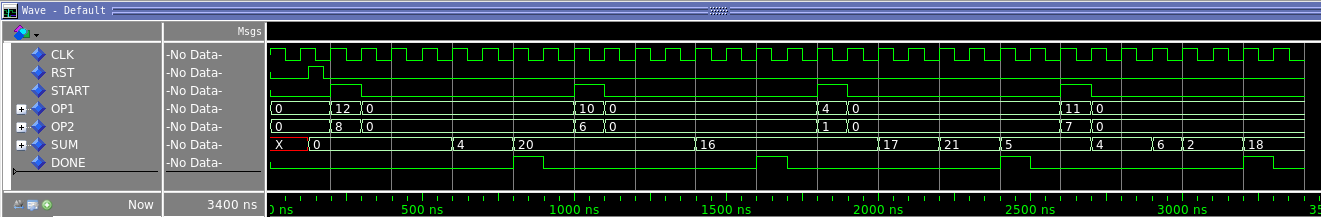
\includegraphics[width=\textwidth]{figs/waveform_sequential_process_automatic_termination.png}
                    \caption{Automatic termination}
                    \label{fig:waveform_sequential_process_automatically_terminates}
                \end{centering}
            \end{figure}

        \end{subsubsection}
    \end{subsection}

\end{section}

%=============================================================================
\end{document}
